\documentclass[•]{beamer}

\title{Face Detection and Recognition}
\author{Meet Gandhi}
\institute{IIT Gandhinagar}
\date{April 17, 2016}
\logo{
\includegraphics[scale=0.1]{iitgnlogo_.png}}

\usetheme{Luebeck}


\begin{document}
\begin{frame}
\titlepage
\end{frame}


\begin{frame}
\frametitle{Various Methods and Algorithms used for Face Detection}
\centering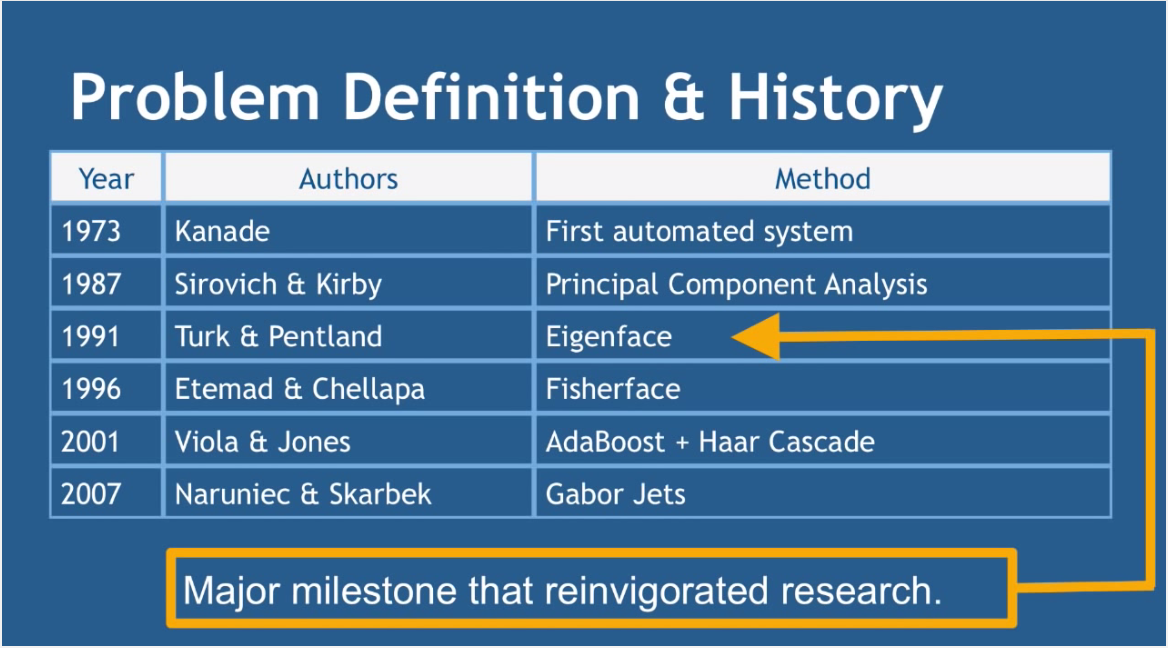
\includegraphics[scale=0.4]{Capture.PNG}
\end{frame}

\begin{frame}
\frametitle{Codes and Concepts}
\setbeamercovered{transparent}

\begin{itemize}%[<+->]
\item<1->{How computers detect faces or separate other things from human faces?}\\
%\pause
\item<2->{By Skin Colour (Colour Detection).}\\
%\pause
\item<3->{Motion(Blinking of Eyes).}\\
%\pause
\item<4->{Head shape and other unique features of the face.}\\
\item<5->{All of the above combined.}\\
\end{itemize}
\end{frame}

\begin{frame}
\setbeamercovered{transparent}
\frametitle{Codes and Concepts}
\begin{itemize}
\item<1->{Most of the modern algorithms for face detection are appearance based rather then learning based.}
\item<2->{Modern face detection algorithms are mostly based on Viola Jones object detection frame work which is based on \bf Haar Cascades.}
\end{itemize}
\end{frame}

\begin{frame}
\setbeamercovered{transparent}
\frametitle{What is a \bf Haar Cascade ?}
\begin{itemize}
\item<1->{Haar Cascade is a collection of Haar like features included altogether to form a classifier.}
\item<2->{Haar like features:}
\end{itemize}
\centering
\includegraphics[scale=0.4]{features1.png}
\end{frame}

\begin{frame}
\setbeamercovered{transparent}
\frametitle{How does Haar like feature function?}
\begin{itemize}
\item<1->{Fix a scale for Haar like feature (For example: 24 X 24 pixels).}
\item<2->{Starting from the topmost left, slide the Haar-like feature across the whole image.}
\item<3->{Calculate the average pixel values in white and black area of the Haar-cascade.}
\item<4->{If the difference of these values is greater than some threshold, the Haar-like feature matches with the portion of the image Haar-like feature is acted upon.}
\end{itemize}
\centering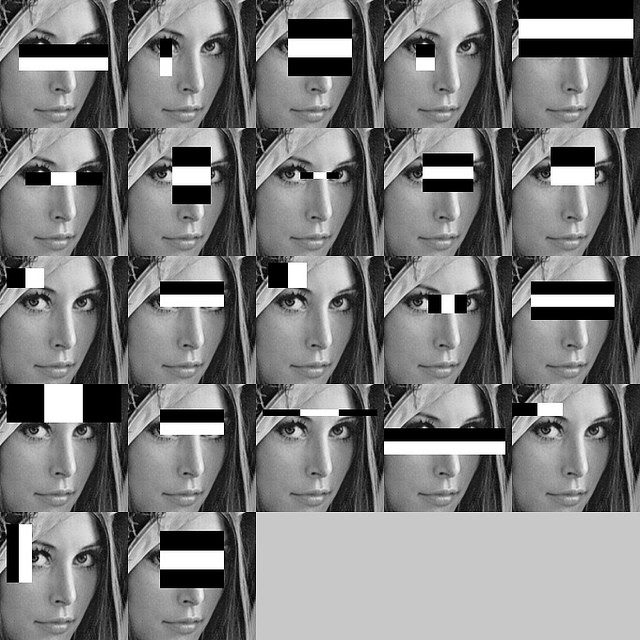
\includegraphics[scale=0.16]{Haar_cascaded.png}
\end{frame}

\begin{frame}
\setbeamercovered{transparent}
\frametitle{Integral Image- A technique to compute the sum of pixels in a given area}
\begin{itemize}
\item<1->{Let the computed pixel values obtained by acting the convoluted kernel on an area of an input image be:}
\item<2->{Summed-Area Table can be computed by adding all the pixel values which are to the left and also up of the given pixel.}
\end{itemize}
\centering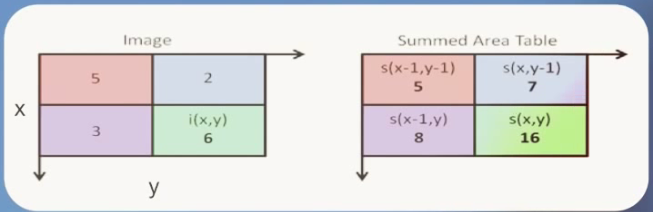
\includegraphics[scale=0.6]{Capture1.PNG}
\end{frame}

\begin{frame}
\setbeamercovered{transparent}
\frametitle{Integral Image- A technique to compute the sum of pixels in a given area}
\centering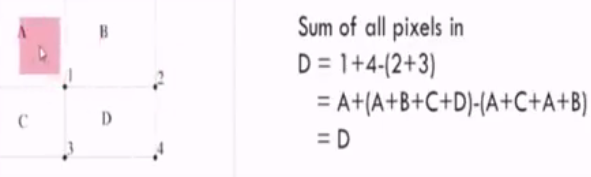
\includegraphics[scale=0.6]{Capture2.PNG}
\begin{itemize}
\item<1->{As a result, Integral Image computation allows to calculate the sum of pixels in a given rectangle by only knowing the pixel values at the corners of the rectangle.}
\end{itemize}
\end{frame}

\begin{frame}
\setbeamercovered{transparent}
\frametitle{Role of Adaboost}
\begin{itemize}
\item<1->{Adaboost is a machine learning algorithm that eliminates the redundant features and finds only the best features which can describe the face among 160,000+ features.}
\item<2->{After these features are found, a linear combination of these features is used to decide whether a window or a photograph has a face or not.These features are known as \bf Weak classifiers.}
\item<3->{Adaboost forms a {\bf Strong classifier} which is a linear combination of weak classifiers.}
\item<4->{Negative value of weighted constant means that the image possesses the opposite feature to that of the Haar-like feature, to some extent which is decided by its magnitude.}
\end{itemize}
\centering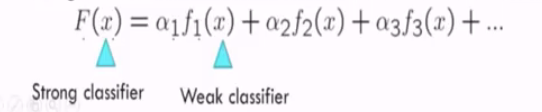
\includegraphics[scale=0.5]{Capture3.PNG}
\end{frame}

\begin{frame}
\setbeamercovered{transparent}
\frametitle{Cascading}
\begin{itemize}
\item<1->{Cascade classifier is made up of stages. Each stage consists of strong classifiers which is the collection of the most covariant features.}
\end{itemize}
\centering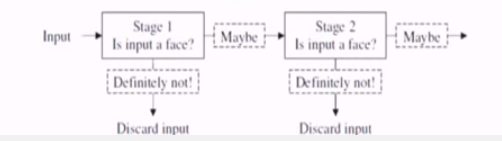
\includegraphics[scale=0.8]{Capture4.PNG}
\end{frame}

\begin{frame}
\setbeamercovered{transparent}
\frametitle{Applications of Face Detection and Recognition}
\begin{itemize}
\item<1->{Attendance System}
\item<2->{Traffic Regulation at 4 Way crossing by counting the number of people through Face Detection and depending on it controlling the green signal}
\item<3->{Modern Digital and Smartphone cameras use Face Detection techniques for autofocus.}
\item<4->{Face Detection and Recognition is used in Biometrics, video surveillance and image database management.}
\end{itemize}
\end{frame}
\end{document}